\begin{figure}[!htbp]
    \centering
    \subfigure[EFFECT OF O.C.R. OCR的作用]{
        \label{figure:11a}
        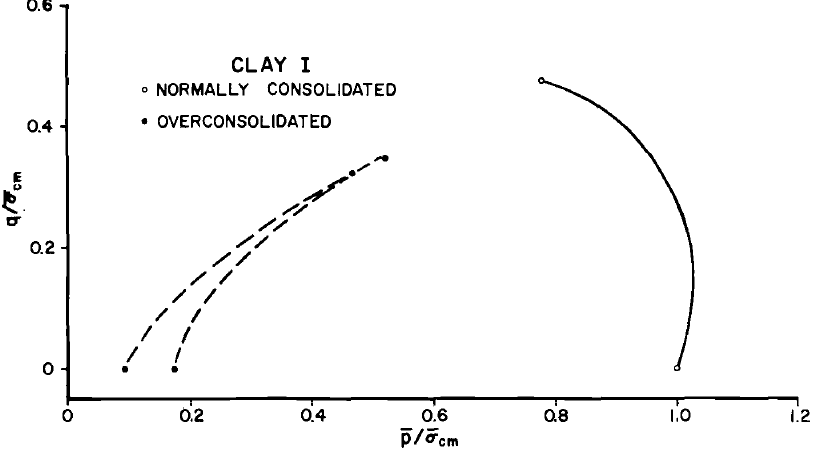
\includegraphics[width=0.48\textwidth]{figures/figure-11a.png}
    }
    \subfigure[EFFECT OF SAMPLING 采样的作用]{
        \label{figure:11b}
        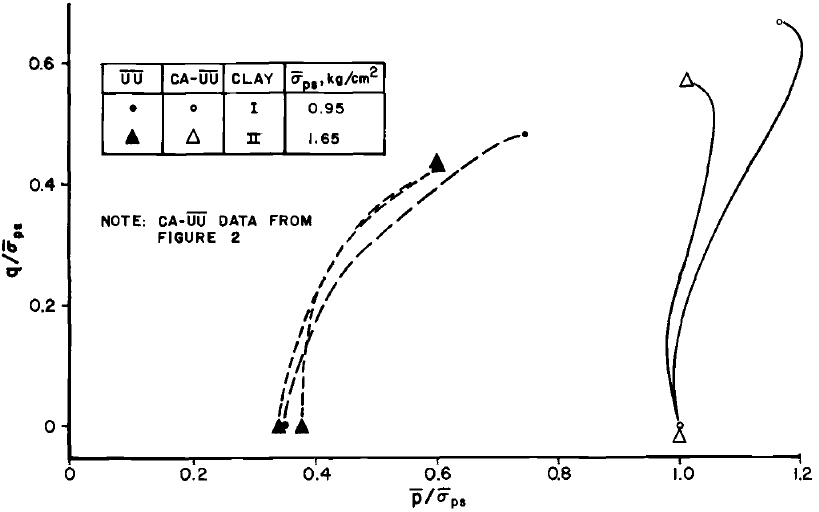
\includegraphics[width=0.48\textwidth]{figures/figure-11b.png}
    }
    \caption{Stress Paths for Kawasaki Clays.}
    \addtocounter{figure}{-1}
    \vspace{-5pt}
    \renewcommand{\figurename}{图}
    \caption{Kawasaki黏土的应力路径。}
    \renewcommand{\figurename}{Figure}
    \label{figure:11}
\end{figure}